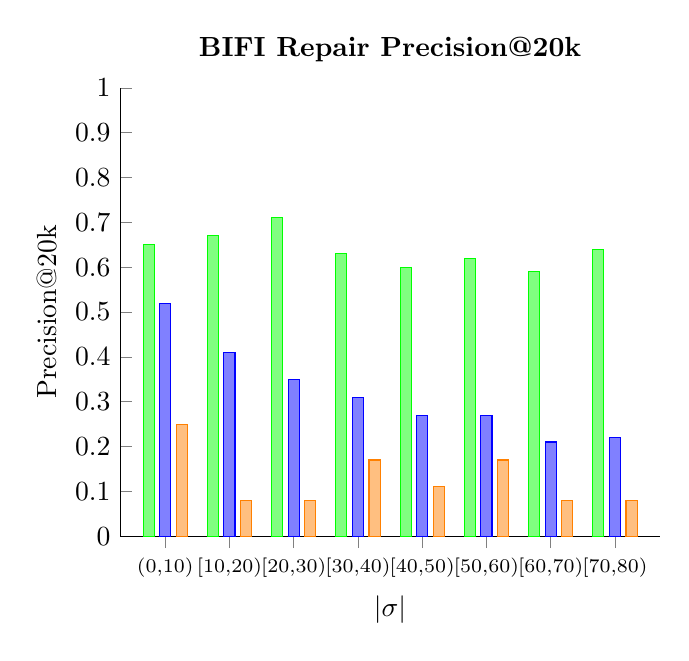
\begin{tikzpicture}
  \begin{axis}[
  xlabel={$|\sigma|$},
  ylabel={Precision@20k},
  title={\textbf{BIFI Repair Precision@20k}},
  ybar,
  axis lines*=left,
  xtick={0, 10, 20, 30, 40, 50, 60, 70},
  ytick={0, 0.1, 0.2, 0.3, 0.4, 0.5, 0.6, 0.7, 0.8, 0.9, 1.0},
  xticklabels={{(}0{,}10{)}, {[}10{,}20{)}, {[}20{,}30{)}, {[}30{,}40{)}, {[}40{,}50{)}, {[}50{,}60{)}, {[}60{,}70{)}, {[}70{,}80{)}},
  x tick label style={font=\scriptsize},
  ymax=1.0,
  ymin=0.0,
  bar width=4pt,
  ]

  \addplot[green, fill=green!50] coordinates {(0, 0.65) (10, 0.67) (20, 0.71) (30, 0.63) (40, 0.6) (50, 0.62) (60, 0.59) (70, 0.64)};
  \addplot[blue, fill=blue!50] coordinates {(0, 0.52) (10, 0.41) (20, 0.35) (30, 0.31) (40, 0.27) (50, 0.27) (60, 0.21) (70, 0.22)};
  \addplot[orange, fill=orange!50] coordinates {(0, 0.25) (10, 0.08) (20, 0.08) (30, 0.17) (40, 0.11) (50, 0.17) (60, 0.08) (70, 0.08)};

  \end{axis}
\end{tikzpicture}
